%!TEX root =  ../samplepaper.tex
\section{Algorithm}
Our algorithm is structured in the three sequential steps discussed in this section.
We next present our algorithm that allows advanced feedback for ND exercises.

%The first step is to generate a hypergraph based on the main goal (what the exercise asks us to prove) and the target goal (the part of the student's proof we want to complete), in order to store all possible rule applications for both goals. Then, we use this graph to build a second hypergraph that simulates as many proof constructions as possible by decomposing the target goal into sub-goals. In the last step, we trim this second graph so that it retains only valid and minimal proofs, either in terms of the number of steps required or the height needed to solve the problem. Finally, we use the resulting graph to extract and build readable proofs, which can later be used to generate feedback.

\subsection{Transition Graph}
\cmt{RG: Estes dois parágrafos inicias precisavam de alguma revisão (em termos de apresentação das ideias), mas não consegui fazer. Posso voltar a isto depois.}
The first step is to create the so-called Transition Graph (TG). This graph stores the formulas that might be part of the final proof, as well as the rules that can be applied to each formula. 
To generate the graph, we need to specify what the consequence we want to prove \(\Gamma \vdash \varphi\), and the target goal \(\Sigma \vdash \theta\), which is the part of a student's proof that needs to be completed. The main goal is used to generate all the natural proof paths, which are proofs built using only formulas derived from decomposing the main goal. The target goal, on the other hand, can sometimes be used to generate non-natural proof paths. By this, we mean proofs that include more complex formulas than those directly derived from the main goal. By considering both goals, the system is able to generate more personalised and user-guided proofs, as it also takes into account the deviations made by the user, which is one of the core elements of our algorithm. For the type of information we want to store, we will make use of a special type of graph~\cite{DBLP:journals/corr/abs-2002-05014}.

\begin{definition}[Labeled Directed Hypergraph with Labeled Heads]
A \emph{Labeled Directed Hypergraph with Labeled Heads} is a pair $H = (V, E)$, where:
\begin{itemize}
  \item \( V \) is a finite set of nodes, and
  \item \( E \subseteq V \times \mathcal{P}(V \times (V \cup \{\varepsilon\})) \times L \) is a finite set of labeled hyperedges, over a finite set of labels $L$, where each hyperedge $(t,\{(h_i,\ell_i): i\in I\}, \ell)$ consists of:
  \begin{itemize}
    \item a tail $t$, representing a single input node from \( V \),
    \item a set of labeled heads, which is a set of pairs \( (h_i, \ell_i) \in V \times (V \cup \{\varepsilon\}) \), where \( h_i \) indicates one of the output nodes and \( \ell_i \) is its label, which is either a node or the empty symbol \( \varepsilon \), and
    \item the global label $\ell$ of the hyperedge, which is an element of \( L \).
  \end{itemize}
\end{itemize}
\end{definition}

The Transition Graph (TG) we will construct is a directed hypergraph as defined above, where vertices are formulas and each hyperedge represents the application of an inference rule, which, as we have seen, may have more than one premise.
%
%
%\begin{definition}[Transition Graph]
%A \emph{Transition Graph (TG)} is a pair
%\[
%T_G = (F, T_E),
%\]
%where:
%\begin{itemize}
%  \item \( F \) is a finite set of \emph{formulas}, and
%  \item \( T_E \subseteq F \times \mathcal{P}(F \times (F \cup \{\varepsilon\})) \times R \) is a finite set of \emph{labeled hyperedges} called \emph{Transition Edge (TE)}, where each edge consists of:
%  \begin{itemize}
%    \item a tail formula \( f \in F \),
%    \item a set of pairs \( (f_1, f_2) \in F \times (F \cup \{\varepsilon\}) \), where \( f_1 \) is a \emph{hypothesis} and \( f_2 \) is a \emph{closed hypothesis}, and
%    \item a rule \( r \in R \).
%  \end{itemize}
%\end{itemize}
%\end{definition}
%
To give some intuition on the formal construction of TG, in \autoref{fig:te-ex} we can see  how the applications of rule \(\vee_E\) can be represented using hypergraphs. Thin edges link head labels, the thick edge links the tail, connected via the dot.



    \begin{figure}[h]
        \centering
        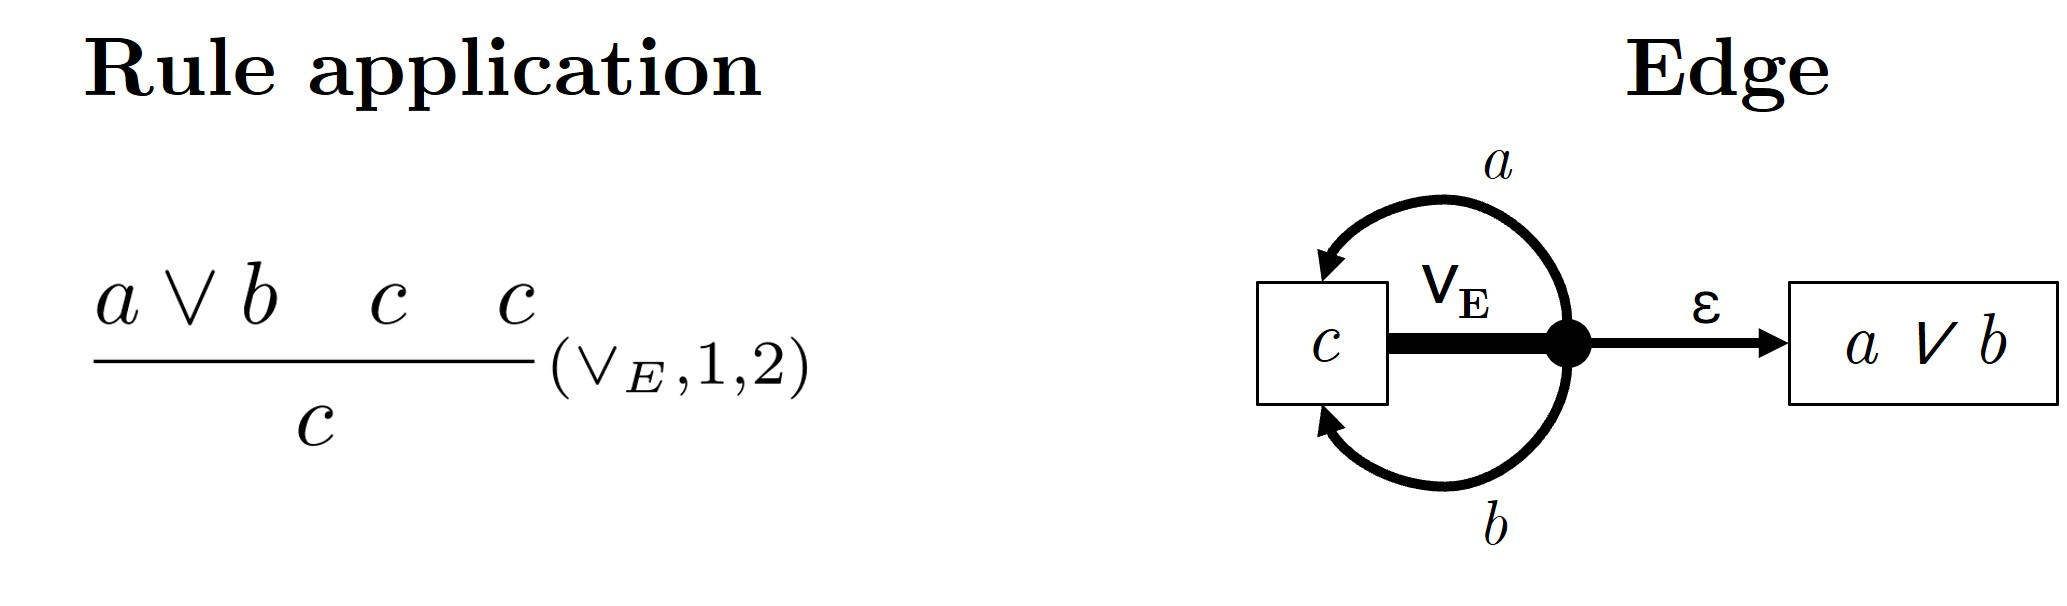
\includegraphics[width=0.7\linewidth]{resources/te-example.jpg}
        \caption{Example of a transition edge. Marks are ignored as irrelevant at this stage. The rule yields only two hypotheses, hence~$\varepsilon$ is needed.}
        \label{fig:te-ex}
    \end{figure}

Formally, the above hyperedge is represented as $(c, \{(a \vee b, \varepsilon), (c, a), (c, b)\}, \vee_E)$. Edges go from the unique conclusion of the rule to its hypotheses. The labels of the heads of the hyperedge represent the possible additional hypothesis that can be used in that branch. In the above rule $\vee_E$, each side of the disjunction can be used as an additional hypothesis in the second and third branches of the rule, encoding the reasoning by cases. 
%If we were working with FOL proofs, we would also need to consider side conditions as part of TG. 
%The reason for using this type of graph is that it allows us to map rule applications directly into a data structure. 
%In the final step, we will explain why it is necessary to store edges in this way. 
%Also, at this point of the construction, there is no need to keep track of the marks. We will see later that we can easily deal with these in the final step of the construction.

%\vspace{1em}
We present, in \autoref{alg:tg-construction}, the concrete procedure to generate the TG.
\begin{algorithm}[h]
\caption{Transition Graph Construction}
\label{alg:tg-construction}
\KwIn{Main goal $\Gamma \vdash \varphi$, Target goal $\Sigma \vdash \theta$}
\KwOut{Transition Graph $T_G = (F, T_E)$}

$F \leftarrow \Gamma \cup \Sigma \cup \{\varphi, \theta\}$\tcp*[r]{Initialize formulas}
$T_E \leftarrow \emptyset$\tcp*[r]{Initialize edges}

\tcp{Compute formulas}
\ForEach{$f \in F$}{
  \If{$f $was not already added as a negation}{
    $F \leftarrow F \cup \{\lnot f\}$\tcp*[r]{Add negation for indirect rules}
  }

  Decompose $f$ into parts $S$\tcp*[r]{The set of sub-formulae of f}
  $F \leftarrow F \cup S$\;
}

\tcp{Compute transitions}
\ForEach{$f \in F$}{
    
    \If{$f$ was not added as a negation}{
        $T_E = T_E \cup \{(f, \{(\bot, \lnot f)\}, \bot)\}$\;
    }

    \If{$f = \lnot \alpha$ for some $\alpha$}{
        $T_E = T_E \cup \{(\lnot \alpha, \{(\bot, \alpha)\}, \lnot_I)\}$\;
        $T_E = T_E \cup \{(\bot, \{(\alpha, \varepsilon), (\lnot \alpha,\varepsilon)\}, \lnot_E)\}$\;
    }

    \ElseIf{$f = \alpha \lor \beta$ for some $\alpha, \beta$}{
        $T_E = T_E \cup \{(f, \{(\alpha, \varepsilon)\}, \vee_{I_R})\}$\;
        $T_E = T_E \cup \{(f, \{(\beta, \varepsilon)\}, \vee_{I_L})\}$\;
        \ForEach{$f' \in F$}{
            $T_E = T_E \cup \{(f', \{(f, \varepsilon), (f',\alpha), (f', \beta)\}), \vee_E\}$\;
        }
    }

    \ElseIf{$f = \alpha \land \beta$ for some $\alpha, \beta$}{
        $T_E = T_E \cup \{(\alpha \land \beta, \{(\alpha, \varepsilon), (\beta,\varepsilon)\}, \land_{I})\}$\;
        $T_E = T_E \cup \{(\alpha, \{(\alpha \land \beta, \varepsilon)\}, \land_{E_R})\}$\;
        $T_E = T_E \cup \{(\beta, \{(\alpha \land \beta, \varepsilon)\}, \land_{E_L})\}$\;
    }

    \ElseIf{$f = \alpha \to \beta$ for some $\alpha, \beta$}{
        $T_E = T_E \cup \{(\alpha \to \beta, \{(\beta, \alpha)\}, \to_{I})\}$\;
        $T_E = T_E \cup \{(\beta, \{(\alpha, \varepsilon), (\alpha \to \beta, \varepsilon)\}, \to_{E})\}$\;
    }

}

\end{algorithm}
As we said, we have as input the consequence we aim to prove \(\Gamma \vdash \varphi\) and a consequence \(\Sigma \vdash \theta\) representing a partial proof of an user. The computation of the relevant formulas and transitions between these can be done in just one loop, but, for the sake of simplicity of presentation, we kept these separated. For the formulas we just consider the set of all subformulas of the formulas contained in the consequence we want to prove and in the partial consequence, together with the negation of these formulas. This way, all formulas that could appear in ND proof of the main consequence are vertices of TG.
The hyperedges of TG correspond to the possible rule applications between these considered formulas.

%The decomposition step is an important part to know in advance which formulas we will have in the graph and also to match with formulas that require that information, since they can be applied to every formula, such as the Elimination of Disjunction rule. The decomposition is done by splitting the formula at the outermost logical operators (if it is not an atomic formula). For example, $a \to \lnot b$ can be split into $a$ and $\lnot b$, but $a$ cannot be decomposed since it is atomic. However, we can decompose $\lnot b$ into just $b$.

To illustrate the construction process, we present a full example in \autoref{fig:tg-final}. The main consequence and the partial consequence are both \(\vdash a \to a\).
\cmt{RG: Não percebo qual é o input neste caso: qual a main consequence e a partial consequence?}
\cmt{DM: Neste caso são o mesmo, por outras palavras, estamos a computar uma solução completa para o problema e não necessariamente a gerar feedback para um passo incompleto de uma prova, por isso main e partial = \(\vdash a \to a\). A minha ideia era ter feito um exemplo em que, de facto, se completasse uma prova mas o numero de nos e arestas cresce demasiado e nao consigo representar o grafo mesmo sendo um pequeno desvio ex: \(\{\lnot (a \to a)\} \vdash a \to \bot\) já ficamos com 6 nos e 12 edges}
\begin{figure}[h]
    \centering
    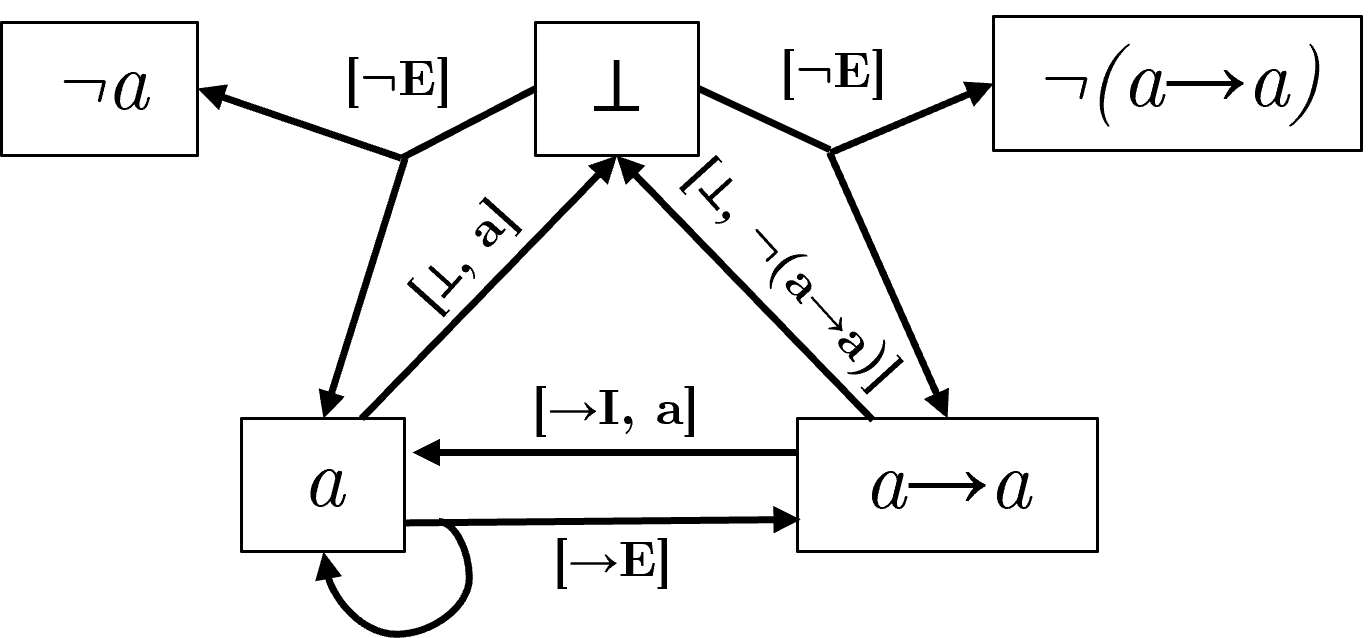
\includegraphics[width=0.8\linewidth]{resources/tg-final.png}
    \caption{Final TG generated from main goal and target goal \(\vdash a \to a\)}
    \label{fig:tg-final}
\end{figure}

\subsection{Proof Graph}
The second step is to build the Proof Graph (PG). The construction of a Proof Graph follows a similar reasoning to the TG, but it is defined on sequents (goals). It contains all possible sub-goals derived from the target goal. In this graph, nodes are goals, and edges are adaptations of transition edges (TE) that now refer to goals. 
%
The purpose of this graph is to decompose the target goal into smaller goals that are easier to prove, until we reach goals that can be directly proved. In the end, after generating all sub-goals, the graph may contain multiple proof paths. 
%
Some of these paths may not lead to a solution, while others may succeed in proving the target goal. In short, the PG aims to find the maximum number of different ``game'' combinations. To generate the PG, we use the TG, previously generated, and the target goal. Note that the target goal can also be the initial goal, in case we want to generate a full proof for the problem. Before we describe the procedure, we define some key terms:

\begin{definition}[Proof Graph]
A \emph{Proof Graph (PG)} is a pair $P_G = (G, P_E)$:
\begin{itemize}
  \item \( G \) is a finite set of \emph{goals}, and
  \item \( P_E \subseteq G \times \mathcal{P}(G \times (F \cup \{\varepsilon\})) \times R \) is a finite set of \emph{labeled hyperedges} called \emph{Proof Edge (PE)}, where each edge consists of:
  \begin{itemize}
    \item a tail goal \( g \in G \),
    \item a set of pairs \( (g_1, f_1) \in G \times (F \cup \{\varepsilon\}) \), where \( g_1 \) is a goal and \( f_1 \) is a \emph{closed hypothesis}, and
    \item a rule \( r \in R \).
  \end{itemize}
\end{itemize}
\end{definition}

\begin{definition}[Proved Goal]
A goal \( \Delta \vdash \delta \) is \emph{proved} if either:
\begin{itemize}
  \item \( \delta \in \Delta \), or
  \item there exists a Proof Edge \( (g, T, r) \in P_E \) in the Proof Graph \( P_G = (G, P_E) \), such that \( g = \Delta \vdash \delta \), and for every pair \( (g_1, f_1) \in T \), the goal \( g_1 \) is proved.
\end{itemize}
\end{definition}

The definition of proved goal is extremely important because it is used as a stopping condition to avoid the algorithm looping through unnecessary goals and to guarantee that the proof is valid. This is only possible due to the type of graph chosen, as it allows us to capture the relation between the hypotheses and the conclusion of each rule application. \autoref{fig:pe-ex} shows an example of a PE and how these relations can be captured. In the figure, we want to prove \(\{a \vee b\} \vdash a\). By applying the Elimination of Disjunction rule, we notice that one of the hypotheses cannot be closed using only this rule, even if the other two hypotheses are closed. So, what we actually prove with this rule is \(\{a \vee b, a\} \vdash a\), which is different from our goal. To accurately track proved goals and only valid proved goals, we must organize goals in a hypergraph structure.

\begin{figure}[h]
    \centering
    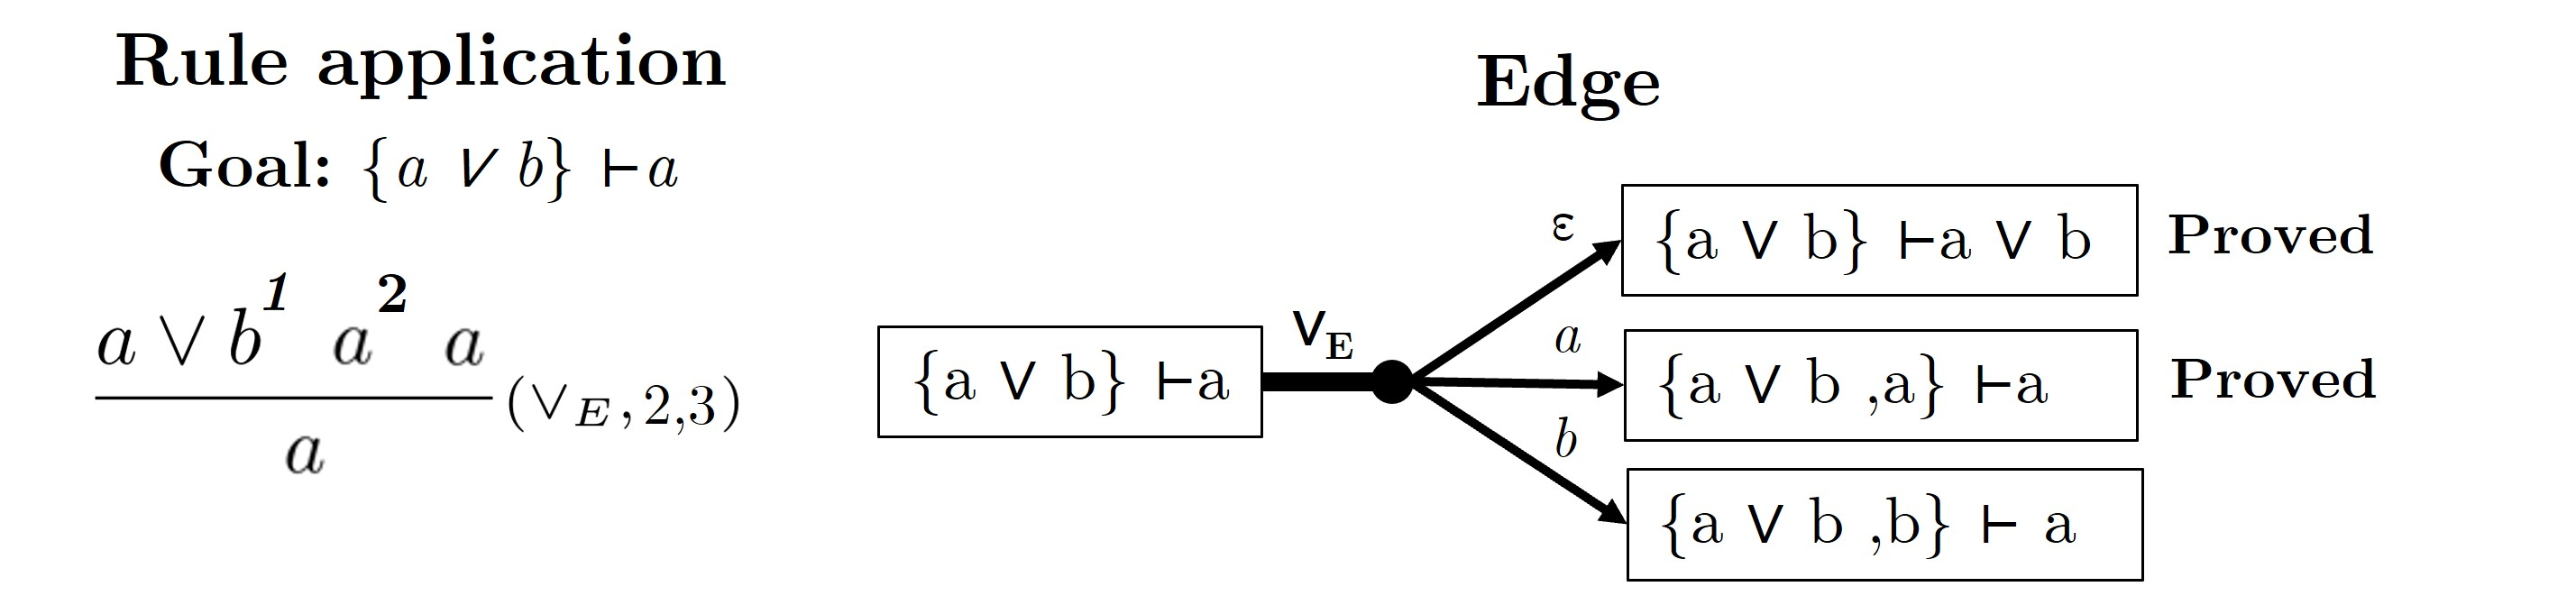
\includegraphics[width=1\linewidth]{resources/pe-example.jpg}
    \caption{Proof attempt of $\{a \lor b\} \vdash a$, no valid proof found.}
    \label{fig:pe-ex}
\end{figure}

\vspace{1em}
With all the necessary definitions in place, we now present the procedure to generate the PG, as shown in \autoref{alg:pg-construction}.

\begin{algorithm}
\caption{Proof Graph Construction}
\label{alg:pg-construction}
\KwIn{Transition Graph $T_G = (F, T_E)$, Target goal $t_\text{goal}$}
\KwOut{Proof Graph $P_G = (G, P_E)$}

$G \leftarrow \{t_\text{goal}\}$\tcp*[r]{Initialize set of goals}
$P_E \leftarrow \emptyset$\tcp*[r]{Initialize set of proof edges}

\tcp{Compute sub-goals}
\ForEach{$g = \Sigma \vdash \theta \in G$}{

    \If{$g$ is proved}{
        \textbf{continue}\tcp*[r]{Skip proved goal}
    }

    \If{stopping condition is reached}{
        \textbf{break}\tcp*[r]{Avoid excessive expansion}
    }

    \tcp{Get transition edges for formula $\theta$}
    $TE_\theta \leftarrow \{ (f, H, r) \in T_E \mid f = \theta \}$\;

    \ForEach{$(f, H, r) \in TE_\theta$}{
        $T \leftarrow \emptyset$\tcp*[r]{Store transitions to each hypothesis}
        
        \ForEach{$(f_1, f_2) \in H$}{
            \tcp{Create sub-goal by extending the current premises with the closed hypothesis}
            $g_\text{new} \leftarrow (\Sigma \cup \{f_2\}) \vdash f_1$\;

            $T \leftarrow T \cup \{(g_\text{new}, f_2)\}$\;
            $G \leftarrow G \cup \{g_\text{new}\}$\tcp*[r]{Add sub-goal}
        }

        $P_E \leftarrow P_E \cup \{(g, T, r)\}$\tcp*[r]{Add proof edge}
    }
}
\end{algorithm}

This algorithm generates very large graphs, with numerous distinct goals depending on the complexity of the problem, especially when dealing with FOL, as it is undecidable. In a pedagogical context, since the size of the proofs we are considering is small, it is not necessary to explore the entire goal space, as many goals are extremely complex and do not provide useful feedback. Therefore, stopping conditions are required, and these depend on the complexity of the specific exercise. These may include limiting the total number of goals explored, setting a maximum number of hypotheses allowed per goal, or enforcing a timeout. The algorithm will find a solution if there is one and no limits are set, but it might take a lot of time and memory.

\autoref{fig:st-ex} shows the PG generated using the TG from \autoref{fig:tg-final} and target goal \(\vdash a \to a\), with a limit of 9 goals explored. Nodes with solid borders represent proved goals, while nodes with dashed borders represent unproved goals. Since our target goal is proved, we know that at least one solution was found.

\begin{figure}[t]
    \centering
    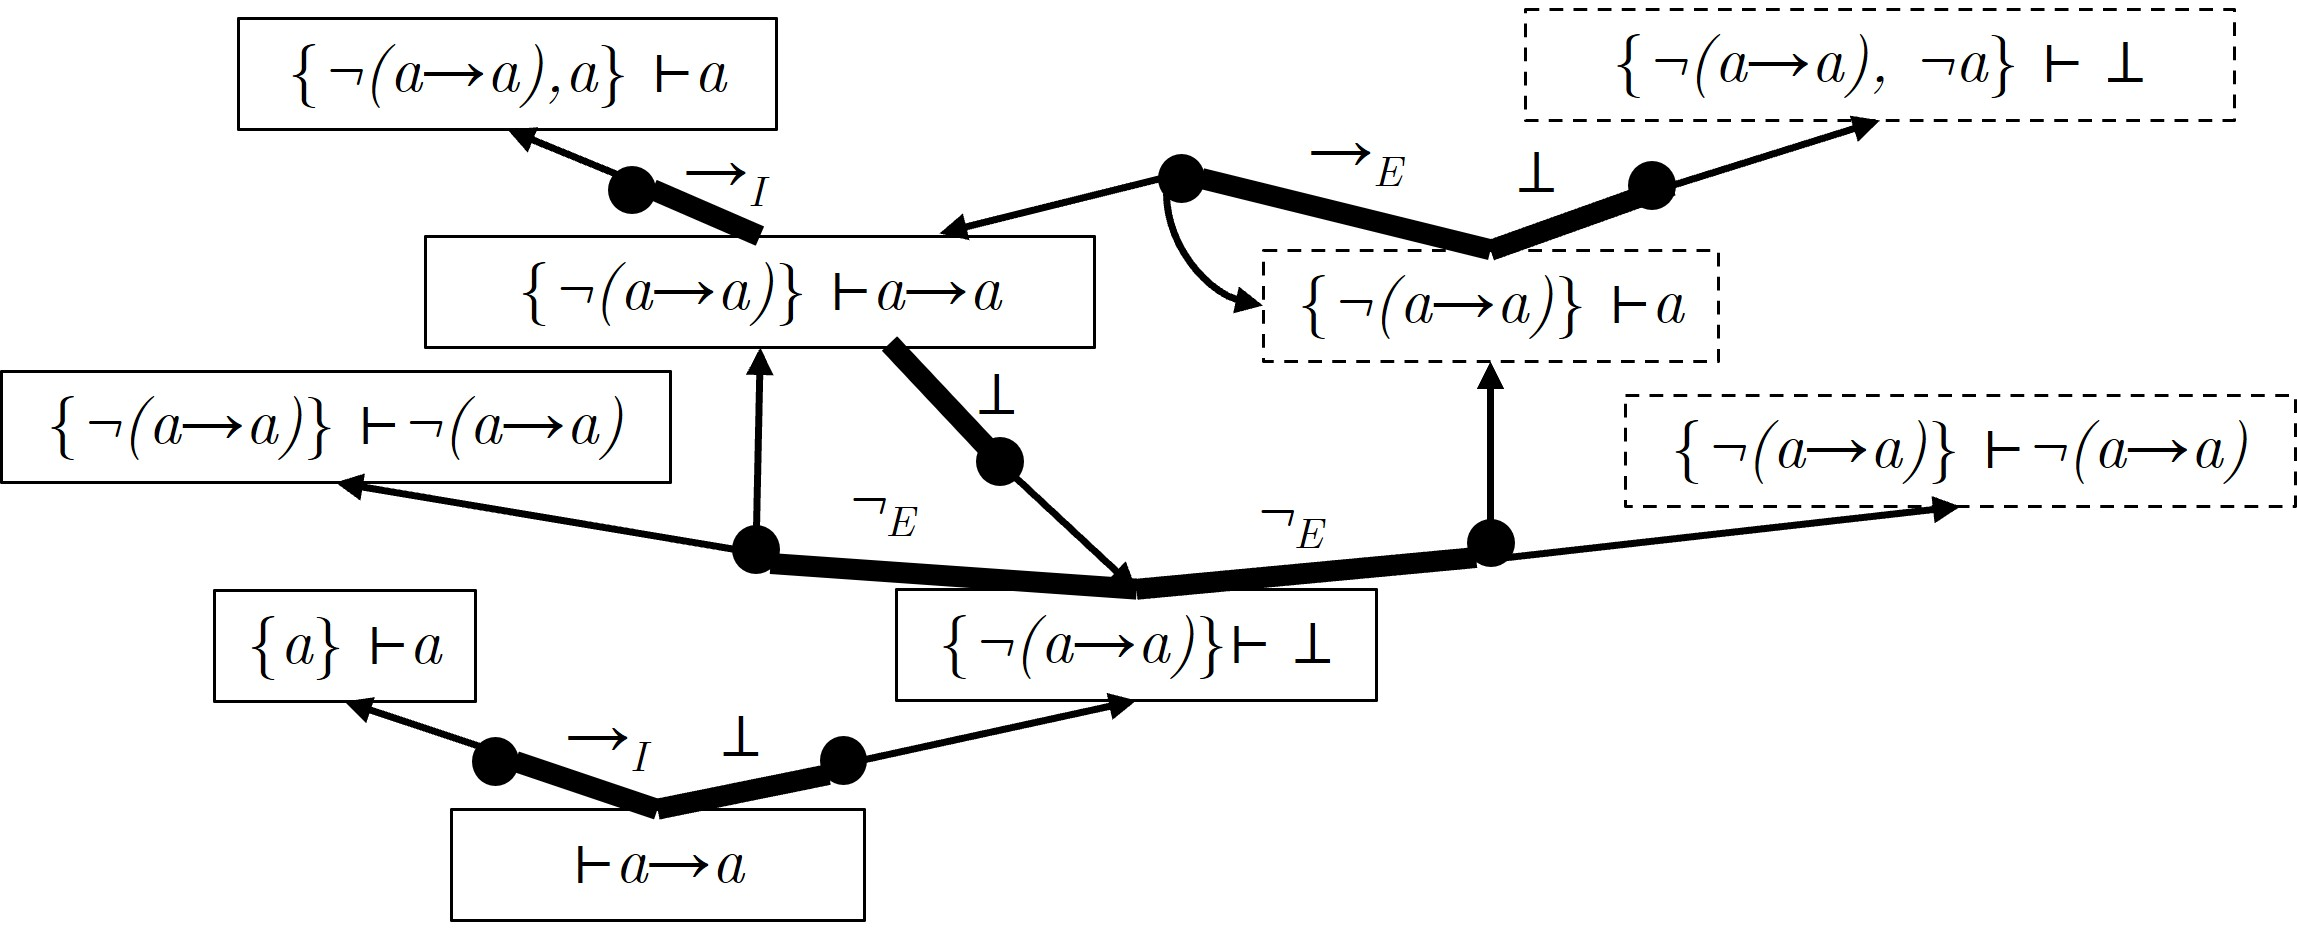
\includegraphics[width=0.8\linewidth]{resources/sg-gen.jpg}
    \caption{Example of a Proof Graph using the TG from \autoref{fig:tg-final} and target goal \(\vdash a \to a\)}
    \label{fig:st-ex}
\end{figure}

\subsection{Proof Graph Trimming}

The final stage of our algorithm consists of trimming the PG to keep only the valid solutions of the problem. The resulting trimmed graph includes only proved goals and the edges that lead to the shortest proofs, where short proofs can be defined in two different ways: one based on height (Height Trim Strategy), and the other based on the number of formulas involved (Size Trim Strategy). Both strategies rely on a standard graph traversal technique, namely \emph{breadth-first search}, to determine which goals and edges should be preserved. The trimming process begins by iterating through all goals and discarding those that cannot be proved. Then, one of the trimming strategies, described below, is applied:
\vspace{1em}

\textbf{Height Trim Strategy (HTS):} This algorithm traverses the PG in reverse order: it starts from the leaves and visits nodes using breadth-first search. Since this traversal guarantees that each node is first reached through the shortest possible path in terms of height, the algorithm retains only the first PE that reaches each goal. All other incoming edges to the same goal are discarded, even if other solutions exist with the same height (see Fig.~\ref{fig:sg-trim-height}).

\begin{figure}[t]
    \centering
    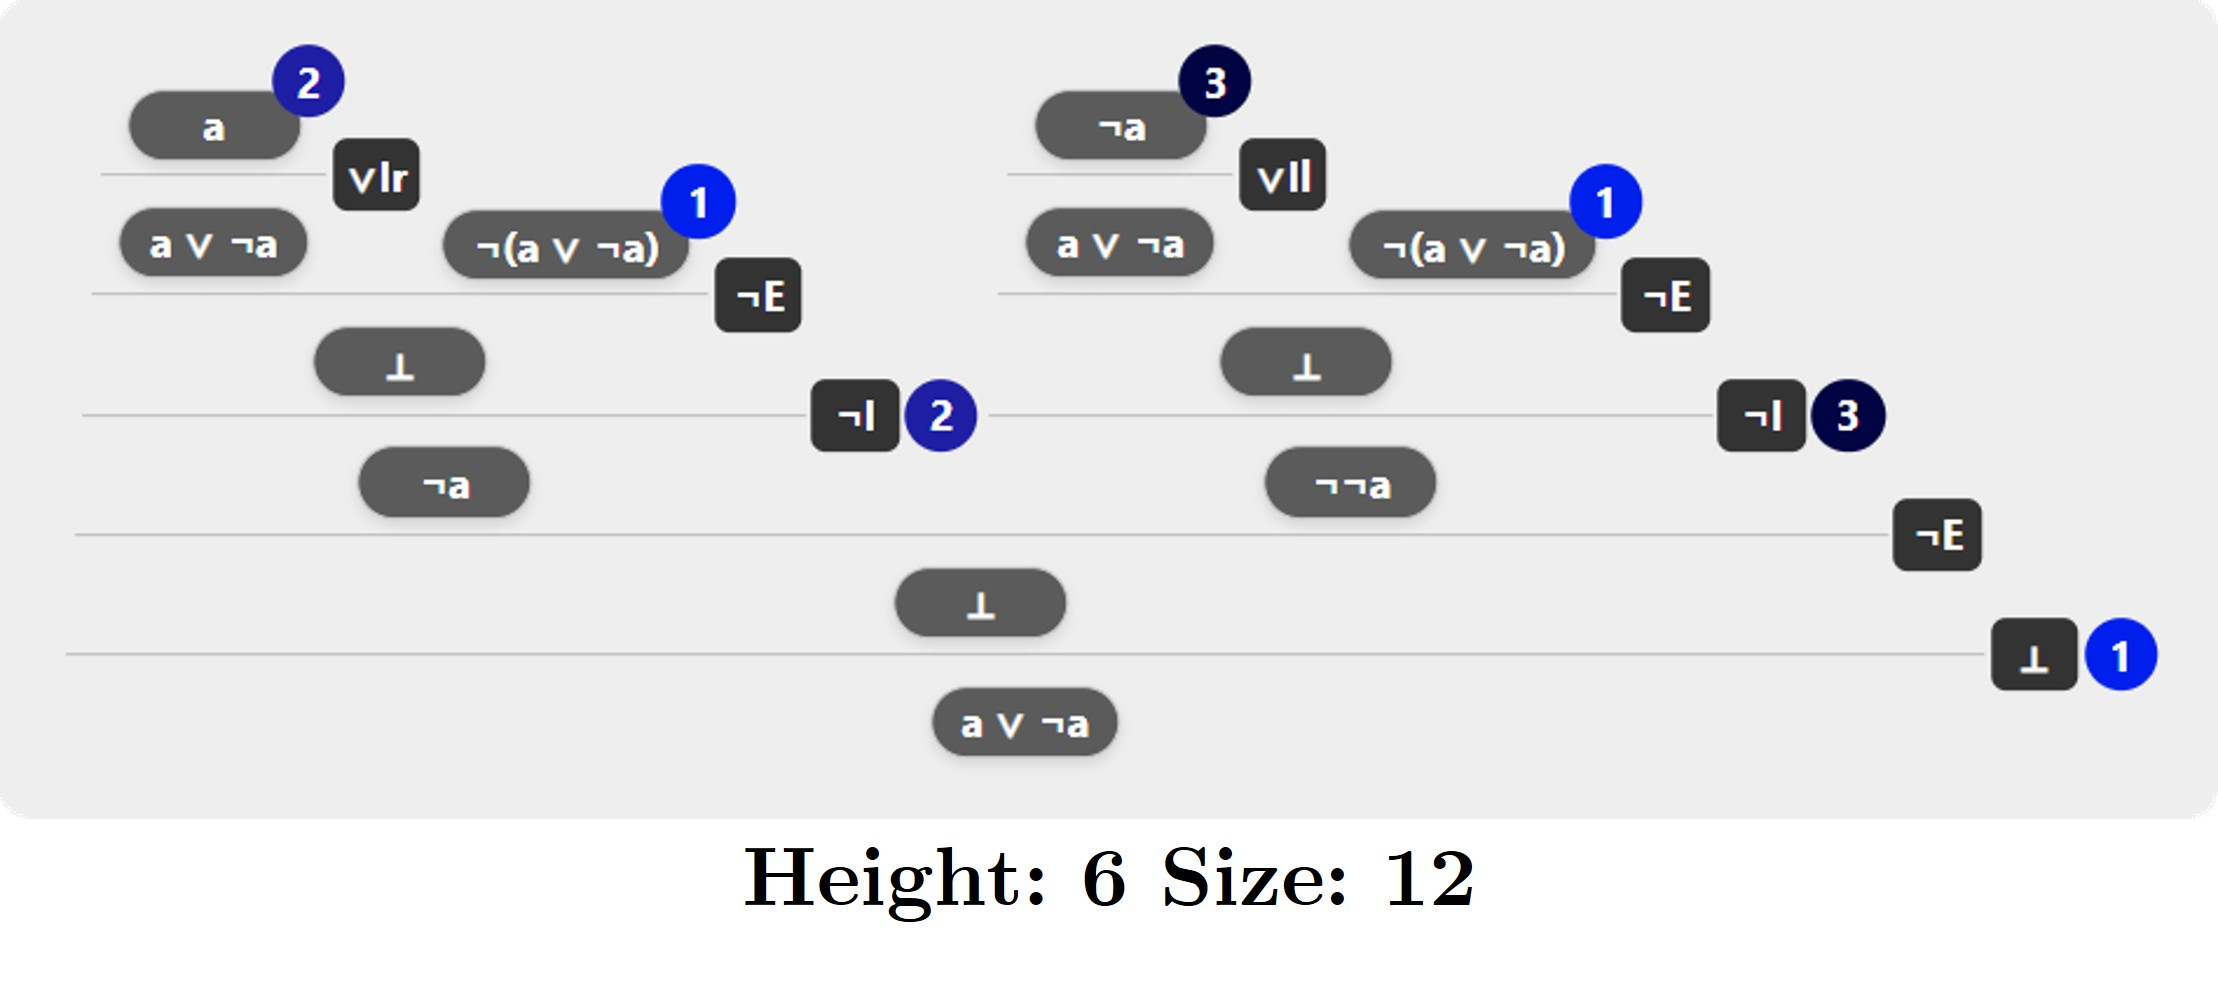
\includegraphics[width=0.6\linewidth]{resources/trim-height.jpg}
    \caption{Example of a full proof generated by the algorithm for \(\vdash a \vee \lnot a\), using HTS.}
    \label{fig:sg-trim-height}
\end{figure}

\textbf{Size Trim Strategy (STS):} This strategy is similar to HTS, but it tracks the size of each proof, defined as the number of formulas involved. Instead of retaining the first edge, it must explore all incoming edges to identify the one that yields the smallest proof. Consequently, a goal may be visited multiple times, making this strategy more computationally expensive. However, it often results in more concise proofs in terms of rule applications (see Fig.~\ref{fig:sg-trim-size}).

\begin{figure}[t]
    \centering
    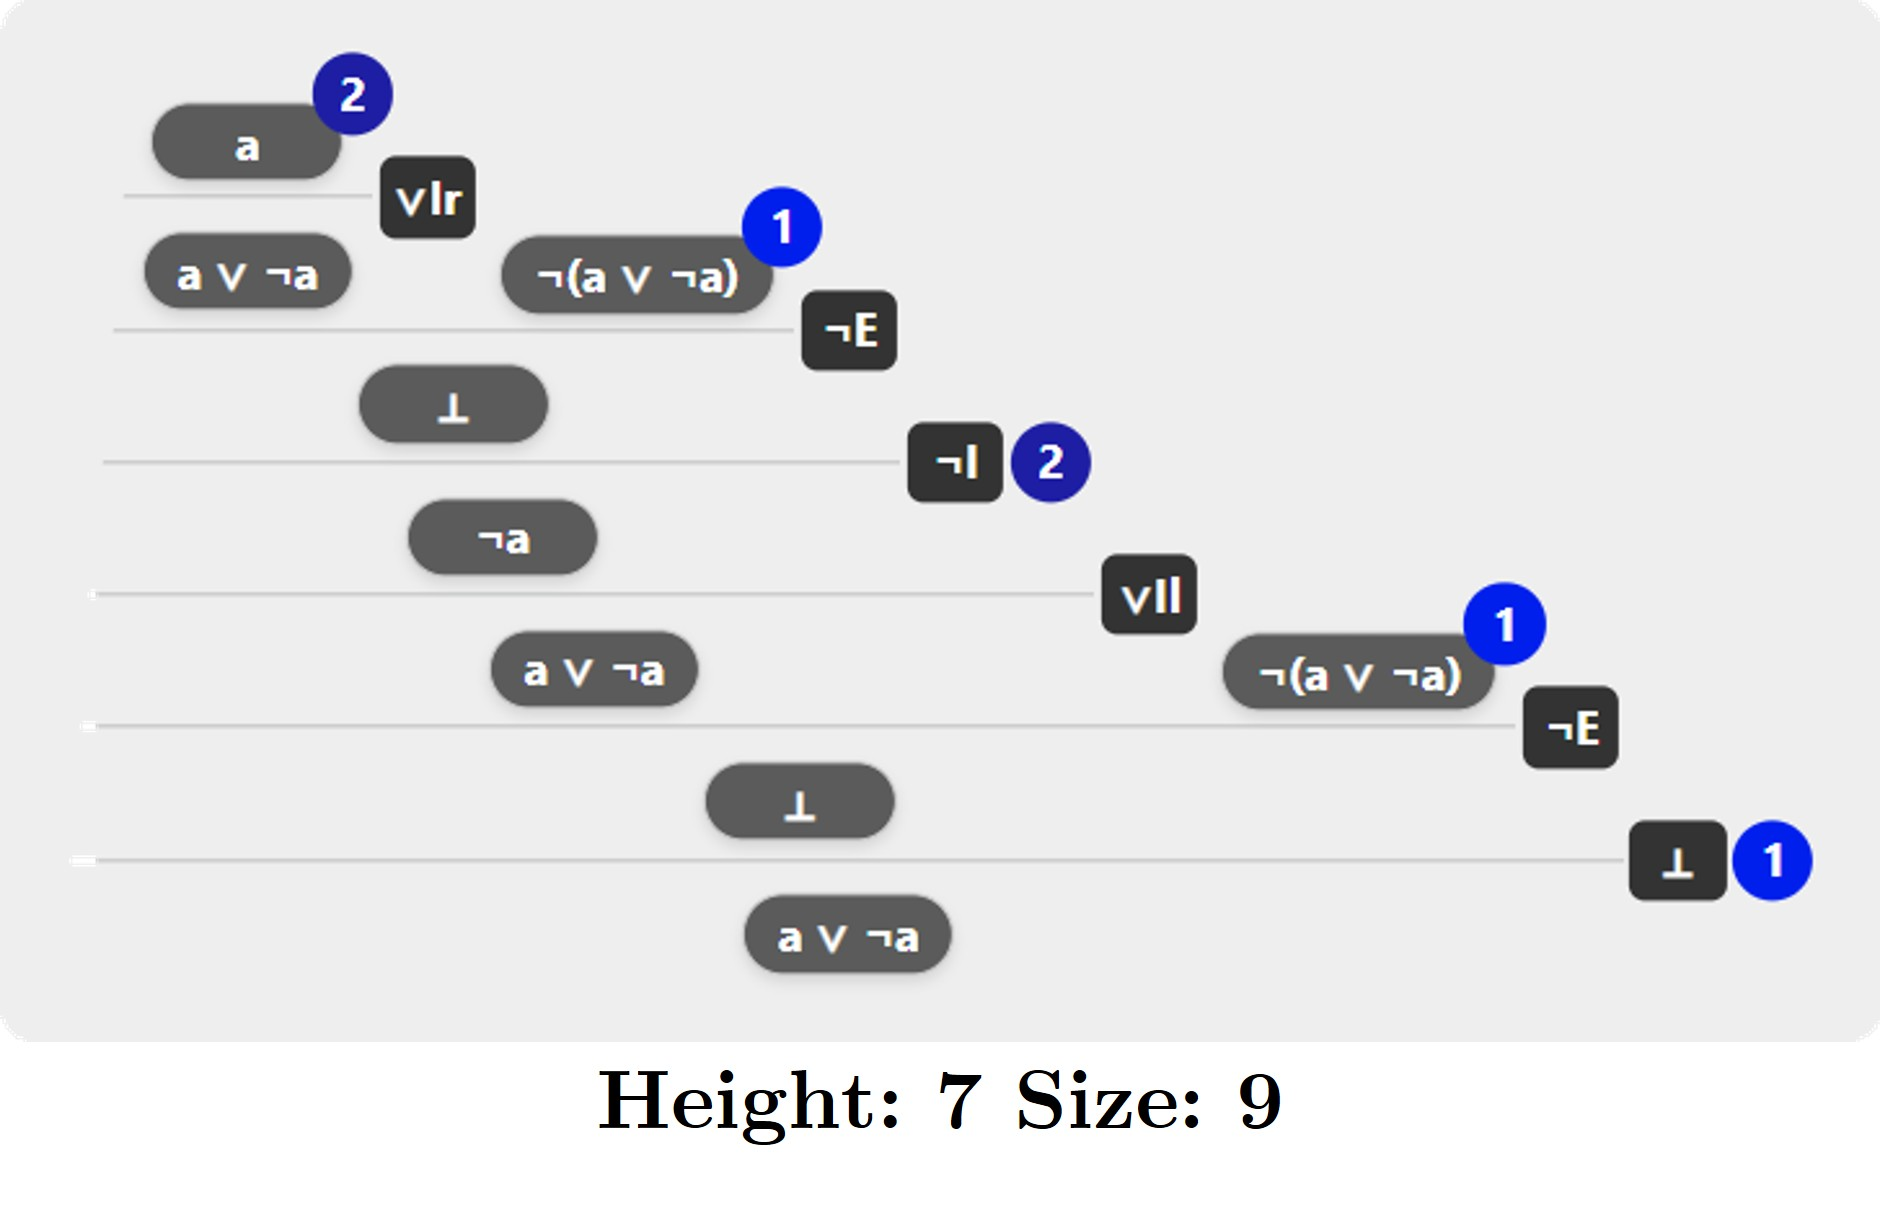
\includegraphics[width=0.6\linewidth]{resources/trim-size.jpg}
    \caption{Example of a full proof generated by the algorithm for \(\vdash a \vee \lnot a\), using STS.}
    \label{fig:sg-trim-size}
\end{figure}

Another key feature that distinguishes our work from other algorithms is that we do not keep just a single solution, but rather a set of possible solutions. This is important to avoid recomputing the entire algorithm when generating feedback for the same problem. However, it comes at a cost in terms of space, as it stores thousands of goals. The algorithm can be queried to generate a new feedback step if all formulas in the new target goal are contained in the set of formulas in the TG used to generate the final trimmed PG. \autoref{fig:sg-trim} shows the TG from \autoref{fig:st-ex} after being trimmed using STS. The algorithm found a solution \textbf{A} for the target problem and also solutions for each of the subgoals presented in the graph.
\begin{figure}[t]
    \centering
    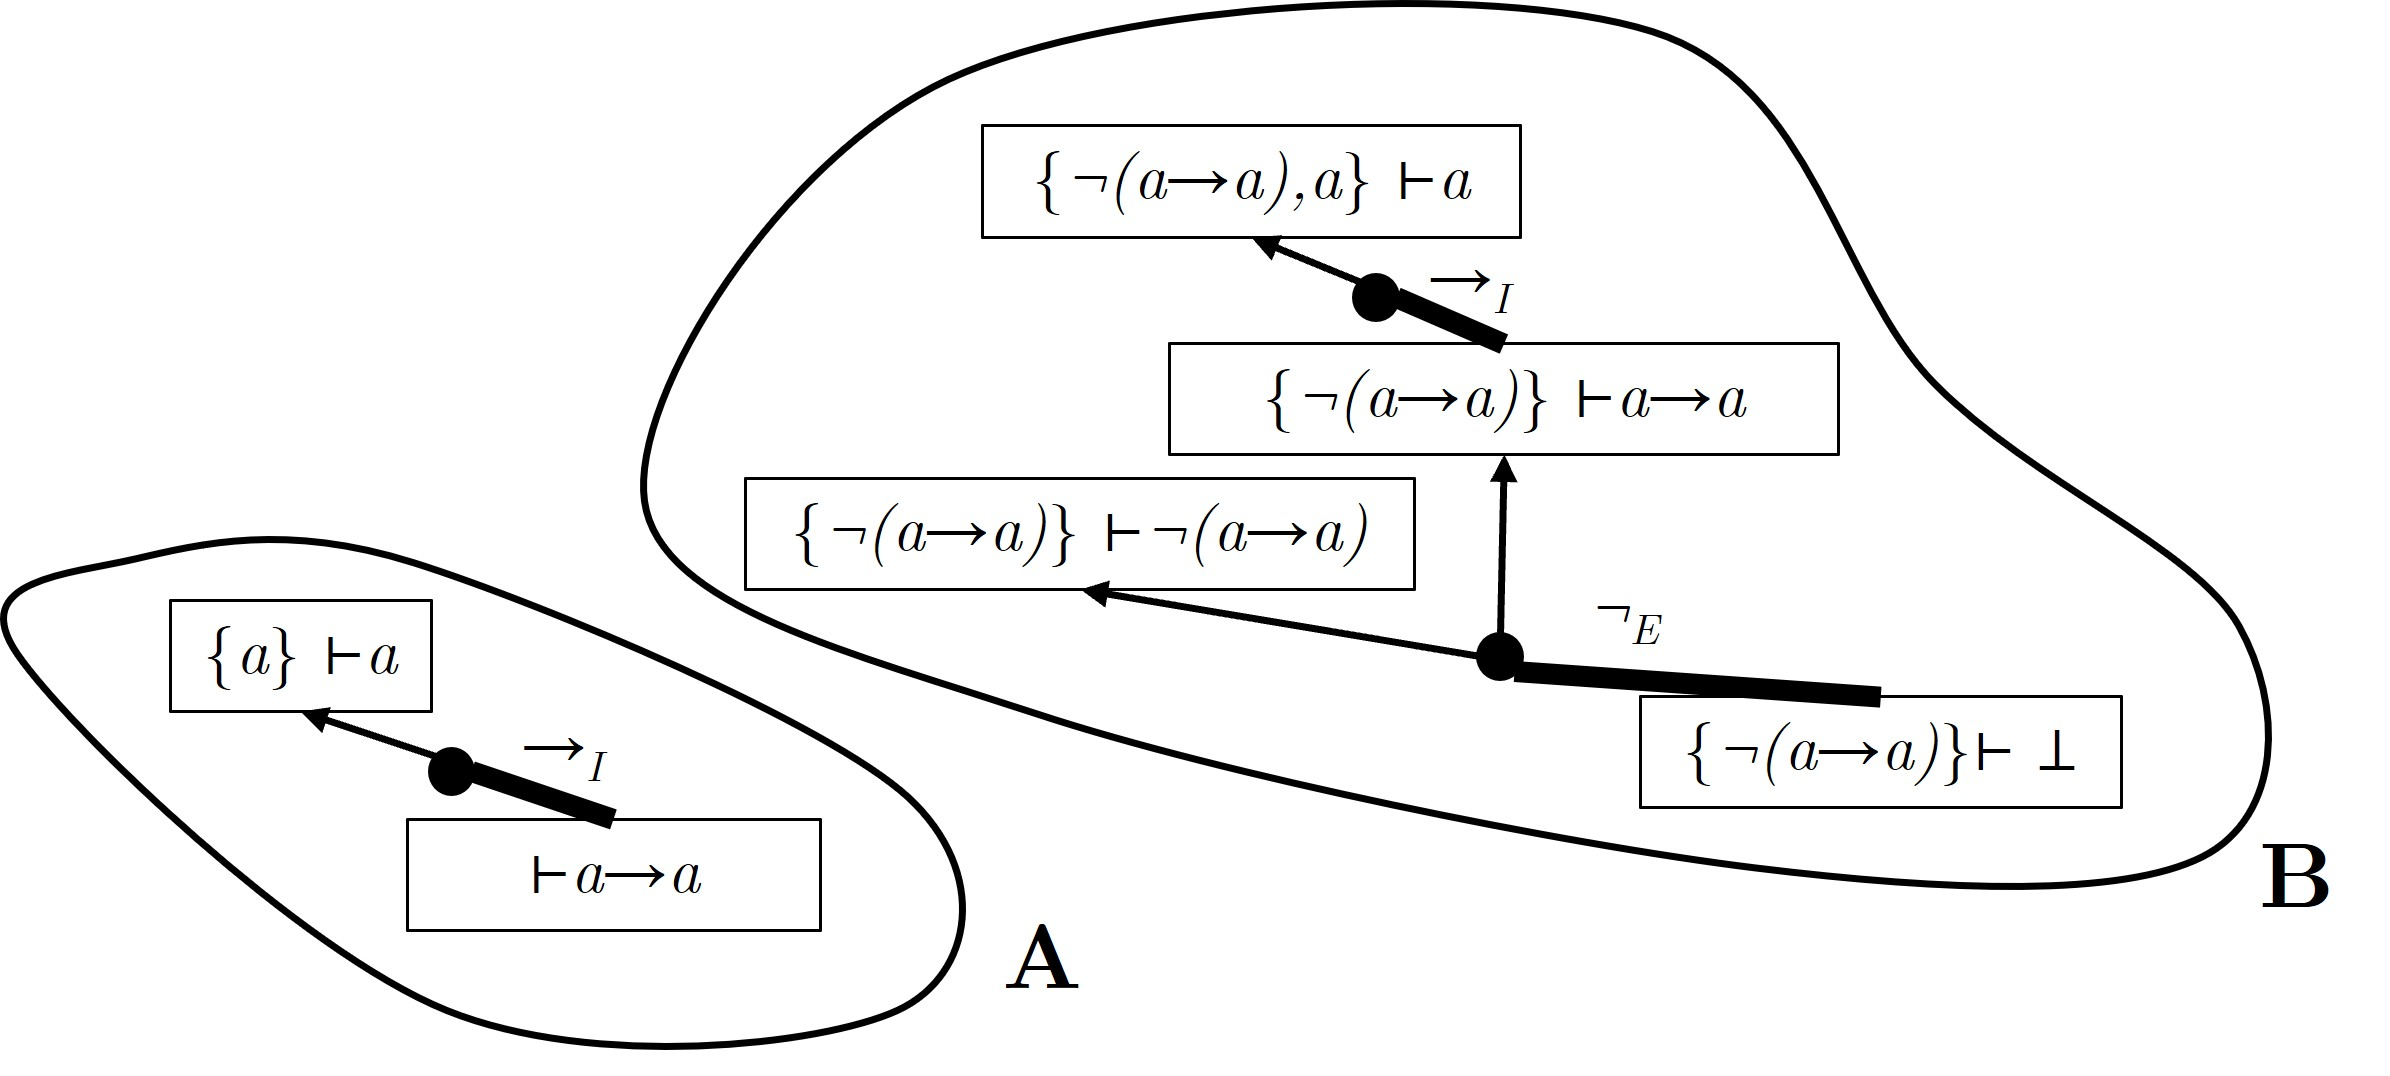
\includegraphics[width=0.8\linewidth]{resources/sg-final.jpg}
    \caption{Trimmed TG using STS.}
    \label{fig:sg-trim}
\end{figure}
\subsection{Feedback Generation}
With the final graph, we can now generate feedback by querying which goals remain unproved in the student's proof. \autoref{fig:extract-solution} and \autoref{fig:extract-solution2} illustrate examples of how feedback can be generated from the final graph.

In this first example, the student does not know how to proceed after applying the Absurdity rule. By querying the  graph with the goal that is still unproved, we get the solution \textbf{B} in \autoref{fig:sg-trim}. Knowing the remaining part of the proof, we can generate feedback. For example, we can tell the student to apply the Elimination of the Negation rule using \(a \to a \) and  \(\lnot(a \to a) \) (cf. objective \textbf{Providing guidance on rule applications} in \autoref{sec:requirements}). In this specific case, we cannot give hints about sub-proofs to solve the problem, as the solution is already small. But in some cases where the solution is bigger, we can do that (cf. objective \textbf{Breaking proofs into smaller sub-proofs}). We can also specify how far the student is from the final proof. In this case, we can say that they are two rules away from completing the proof (cf. objective \textbf{Indicating the distance to a solution}). Finally, we can also suggest some improvements in the resolution. In this case, the student shifts their solution by applying the Absurdity rule, making it longer. That information can also be extracted from the graph (cf. objective \textbf{Improvements in the proof}).

\begin{figure}[t]
    \centering
    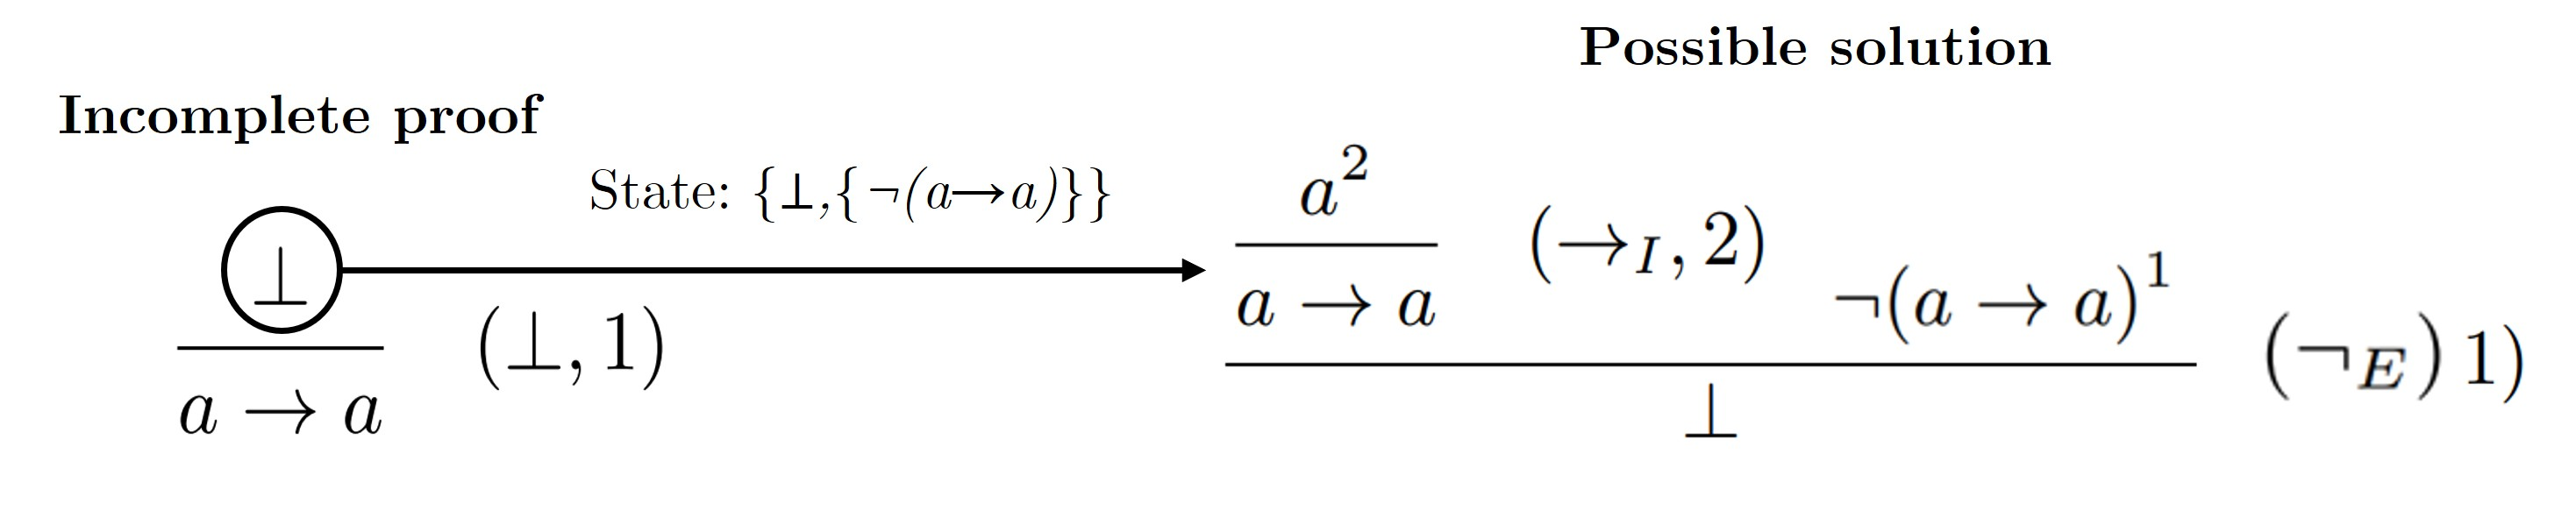
\includegraphics[width=1\linewidth]{resources/trim-pos-feed.jpg}
    \caption{Extracting a solution to produce feedback from a proved goal}
    \label{fig:extract-solution}
\end{figure}

In this second example, a solution cannot be found, as the goal assigned to the unresolved part of the proof does not belong to the final graph. In this case, we can inform the student that the path they are taking may be too complex, and we can suggest going back \(X\) rule applications until the algorithm finds the correct path again to guide the student. We cannot affirm that there is no solution, because we may not have explored the whole space of possible solutions. For example, the final graph was only constructed considering the first 9 nodes. In this example, if the student removes the Elimination of Negation rule (one step back), we return to the situation previously presented.
\begin{figure}[t]
    \centering
    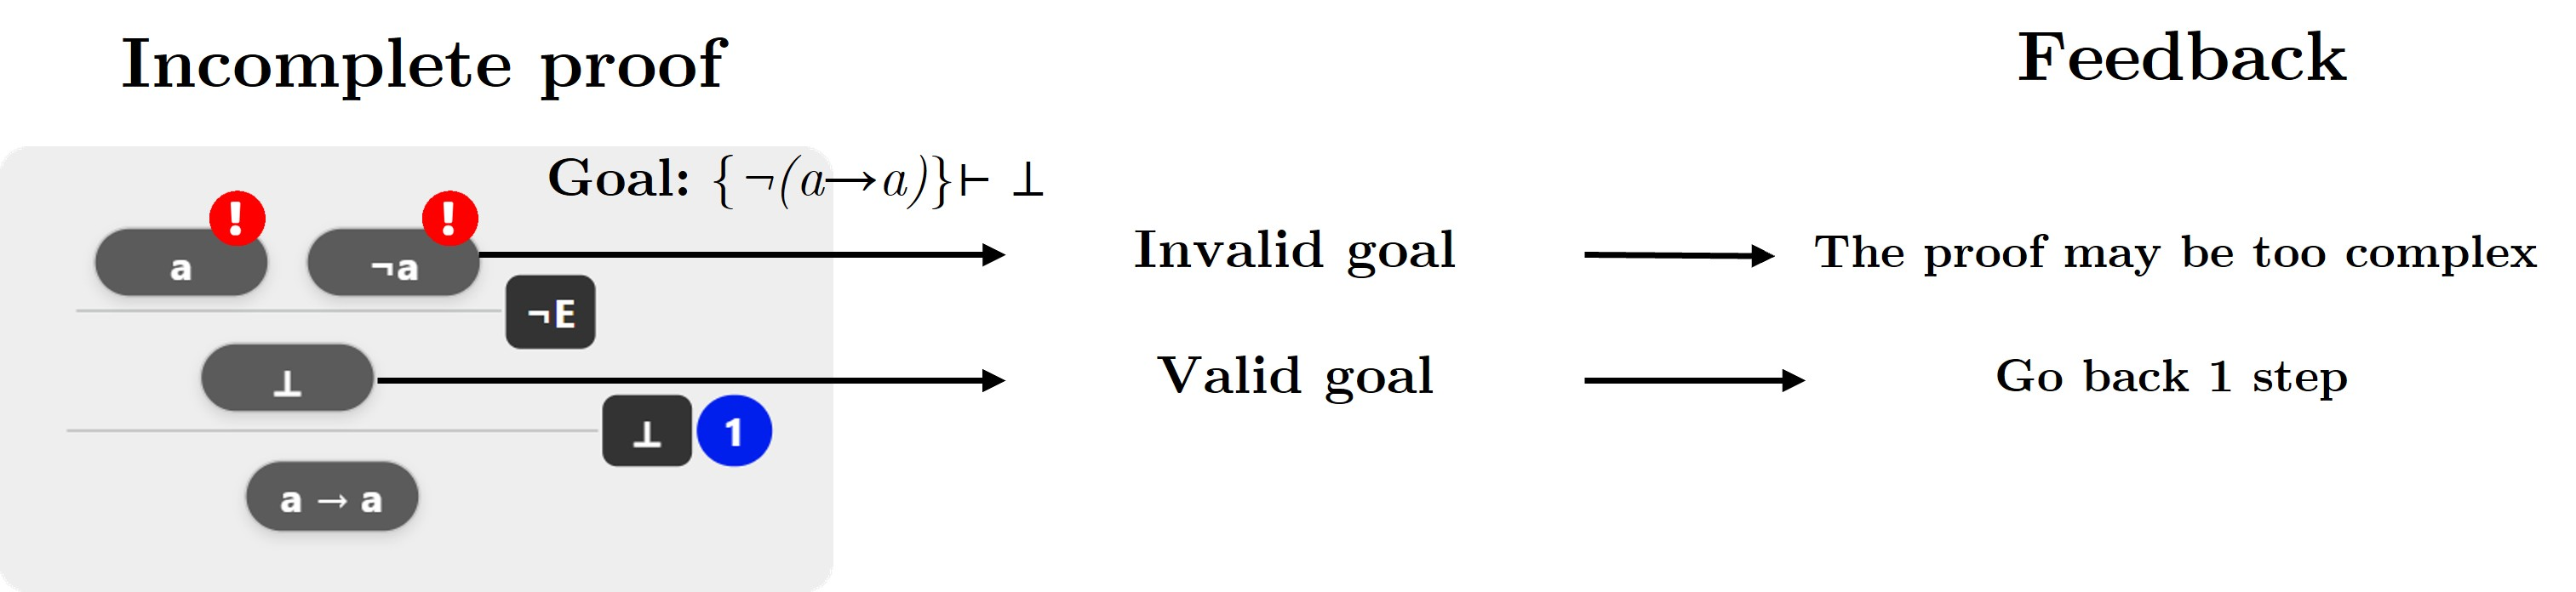
\includegraphics[width=1\linewidth]{resources/trim-neg-feed.jpg}
    \caption{Extracting a solution to produce feedback from an unproved goal.}
    \label{fig:extract-solution2}
\end{figure}
These methodologies can also be used by teachers to assess exercises. For example, we could compute how far a student’s resolution is from a possible solution, or how far it is from the best solution. In some cases, based on the size of the explored solution space, we can say that the student overcomplicated the resolution.

Our algorithm is implemented in a publicly available prototype\footnote{\url{https://github.com/DanielMacau60004/NDAlgorithm}} and has been functionally tested. It is also integrated in a visual online tool focused on ND proofs but still lacks user testing for a proper validation. The figures that include user interaction are captured from the tool that allows students to practice ND proofs.
